\documentclass[11pt, a4paper, twocolumn]{article}


% --- Paquetes de Idioma y Codificación ---
\usepackage[utf8]{inputenc}
\usepackage[spanish, es-nodecimaldot]{babel} % Configurado para español
\usepackage[T1]{fontenc}

% --- Tipografía y Estética ---
\usepackage{mathpazo} % Fuente Palatino, elegante y legible
\usepackage{microtype} % Mejora el espaciado entre letras y palabras

% --- Geometría de Página ---
\usepackage[margin=2.5cm, top=3.8cm, headheight=65pt, headsep=0.8cm]{geometry}
\columnsep 0.6cm % Espacio entre columnas
\usepackage{float}
% --- Matemáticas Avanzadas ---
\usepackage{amsmath, amsfonts, amssymb, amsthm}
\usepackage{mathtools}

% --- Gráficos y Tablas ---
\usepackage{graphicx}
\usepackage{booktabs} % Para tablas con estilo profesional (sin líneas verticales)
\usepackage{caption}
\captionsetup{labelfont=bf, font=small} % Captions en negrita y pequeñas

% --- Hipervínculos y Referencias ---
\usepackage[colorlinks=true, allcolors=blue]{hyperref}
\usepackage[capitalize]{cleveref} % Referencias inteligentes (ej: Fig. 1)
\usepackage{csquotes} % Requerido por biblatex con babel
\usepackage{biblatex}
\addbibresource{referencias.bib}

% --- Título y Autores ---
\title{\textbf{\Large Fractales: Dimensiones enteras y fraccionarias}}
\author{
    \textbf{Truchado Iniesta, Eduardo}, \textbf{Sanz Rubio, Juan} \\
    \small Grado de Física, UCLM. \texttt{juan.sanz1@alu.uclm.es} \\
    \small Grado de Física, UCLM. \texttt{eduardo.truchado@alu.uclm.es}
}
\date{\small 2 Marzo 2026}


\usepackage{fancyhdr}
%\usepackage{graphicx}

% --- Configuración del Encabezado ---
\pagestyle{fancy}
\fancyhf{} % Limpia encabezado y pie de página
\renewcommand{\headrulewidth}{0.4pt} % Línea horizontal bajo el encabezado

% Imagen a la IZQUIERDA
\fancyhead[L]{
\includegraphics[height=2cm]{logoFCTo.png}}

\fancyfoot[C]{\thepage}


\fancypagestyle{plain}{
    \fancyhf{} % Limpia el estilo plain por defecto
    \fancyhead[L]{
\includegraphics[height=2cm]{logoFCTo.png}} % Mantiene tu logo
    \fancyfoot[C]{\thepage} % Fuerza el número de página
    \renewcommand{\headrulewidth}{0.4pt} % Mantiene la línea
}

% --- Inicio del Documento ---

\begin{document}

\maketitle
\thispagestyle{fancy}

%Resumen

\begin{abstract}
En esta práctica se realizaron medidas de diámetro para diferentes esferoides de masas relativas definidas a partir de 1/8 de dimensión 
de una hoja de papel de cocina completa. Con estas dimensiones se obtuvieron de los siguientes tipos de papel; papel de cocina, 
papel aluminio y papel tipo folio, comprimido ligeramente para alcanzar una forma más esferoidal, masa de masa relativa 1,2,4,8,16,32 y 64. 

\vspace{0.2cm}

A partir de la medida de los diámetros, reañizamos una regresión logarítmica para hallar la pendiente y con ello obtener el valor de la dimensión
fractal que se busca. El resultado obtenido fue un valor promedio cercano a $d\approx 2.5$ variando ligeramente para los esferoides más compactados y menos.
\end{abstract}



\section{Introducción}
No todos los objetos geométricos tienen dimensiones enteras (euclidianas) como clásicamente se ha considerado. Algunos con geometrías complejas se describen matemáticamenete 
como objetos con dimensiones fraccionadas, conocidos como fractales. 

\vspace{0.2cm}

El propósito de este estudio es determinar las propiedades dimensionales de objetas
geométricamente complejos, que en este caso serán esferoides, para determinar como
algunos objetos se pueden describir matemáticamente con dimensiones fraccionarias.

\vspace{0.2cm}

Para realizar esto, se ha utilizado la siguiente relación:

\begin{equation}
    D = K M ^{\frac{1}{d}}
\end{equation}

Donde d es la dimensión fractal, M es la masa del objeto, K es una constante de proporcionalidad y D el diámetro de la esfera considerada. Para
analizar la ecuación de forma lineal pasaremos la ecuación con relaciones en base a elyes de potencias a una lineal usado las propiedades de los
logaritmos. Con esto conseguiremos que la pendiente sea la relacion entre la dimension fractal y la masa. 

\begin{equation}
    \log(D) = \log(K) + \frac{1}{d} \log(M)
\end{equation}

Donde la pendiente es igual a $m = \frac{1}{d}$, por lo que a partir de la regresión 
se puede obtener el valor de la dimensión fractal d.
\section{Objetivos}
Los objetivos propuestos son analizar la influencia del tipo de material y de la forma en la que es compactado en un esferoide para poder 
determinar como afecta a su dimensión fractal. 
\section{Metodología}

Para realizar esta práctica se han utilizado 3 tipos de papel: 
\begin{itemize}
    \item Papel de cocina
    \item Papel aluminio
    \item Papel tipo folio
\end{itemize}

Cada uno de estos ha sido tratado de diferente forma. En el caso del papel de cocina, ha sido compactado suavemente con las manos, 
el papel de aluminio ha sido compactado con las manos también pero de forma más intensa, y el papel de tipo folio ha sido comprimido 
con una bandeja con pesos de entorno a 1 kilo por encima. 

\vspace{0.2cm}

Cabe destacar el tamaño utilizado ya que este se ha vasado en un tamaño original consistente en un aproximado 1/8 de un papel de cocina completo. Así siendo este el 
peso de valor 1 y aumentando este hasta llegar a 64.  
\section{Tratamiento de datos}

A continuación mostraremos las tablas de datos obtenidos. Para cada tipo de papel se han realizado 7 medidas para cada masa de cada pelota
y realizado el promedio de estas medidas para cada una. El error asociado es el error del calibre utilizado para la propia medida, en este caso 0.02mm.

\vspace{0.5cm}

Tabla de datos para papel suave:

\begin{tabular}{ccc}
\hline
   Masa (g) &   $\langle$ D $\rangle$ (mm) & $\bigtriangleup$ D (mm)   \\
\hline
          1 &                        16.14 & $\pm$ 0.02                 \\
          2 &                        23.96 & $\pm$ 0.02                 \\
          4 &                        31.66 & $\pm$ 0.02                 \\
          8 &                        41.5  & $\pm$ 0.02                 \\
         16 &                        48.87 & $\pm$ 0.02                 \\
         32 &                        74.19 & $\pm$ 0.02                 \\
         64 &                       108.4  & $\pm$ 0.02                 \\
\hline
\end{tabular}


\vspace{0.5cm}


Tabla de datos para papel aluminio:

\begin{tabular}{ccc}
\hline
   Masa (g) &   $\langle$ D $\rangle$ (mm) & $\bigtriangleup$ D (mm)   \\
\hline
          1 &                        10.06 & $\pm$ 0.02                 \\
          2 &                        11.91 & $\pm$ 0.02                 \\
          4 &                        17    & $\pm$ 0.02                 \\
          8 &                        20.7  & $\pm$ 0.02                 \\
         16 &                        27.06 & $\pm$ 0.02                 \\
         32 &                        35.87 & $\pm$ 0.02                 \\
         64 &                        53.54 & $\pm$ 0.02                 \\
\hline
\end{tabular}


\vspace{0.5cm}


Tabla de datos para papel comprimido:

\begin{tabular}{ccc}
\hline
   Masa (g) &   $\langle$ D $\rangle$ (mm) & $\bigtriangleup$ D (mm)   \\
\hline
          1 &                        10.79 & $\pm$ 0.02                 \\
          2 &                        15.29 & $\pm$ 0.02                 \\
          4 &                        23.69 & $\pm$ 0.02                 \\
          8 &                        27.53 & $\pm$ 0.02                 \\
         16 &                        35.67 & $\pm$ 0.02                 \\
         32 &                        49.17 & $\pm$ 0.02                 \\
         64 &                        62.14 & $\pm$ 0.02                 \\
\hline
\end{tabular}

\vspace{0.5 cm}

Con estos datos, se realiza una represión lineal para cada tipo de papel así pudiendo analizar la dimensión fractal obtenida. En estas aparece ya calculado el
error asociado a la dimensión fractal, que se ha obtenido a partir de la siguiente fórmula: 
\begin{equation}
    \triangle d = \left | \frac{\partial d}{\partial m} \right | \triangle m = \frac{1}{m^{2}} \triangle m
\end{equation}

\begin{figure}[h]
    \centering
    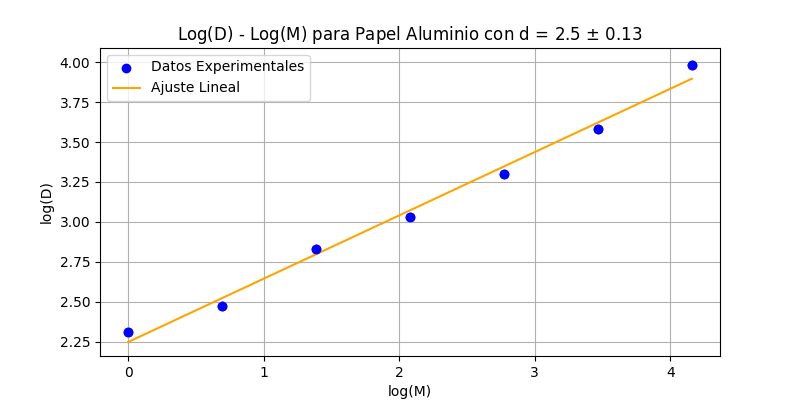
\includegraphics[width=0.4\textwidth]{Papel_aluminio_lineal.png}
    \caption{Regresión lineal para papel aluminio.}
\end{figure}

\begin{figure}[h]
    \centering
    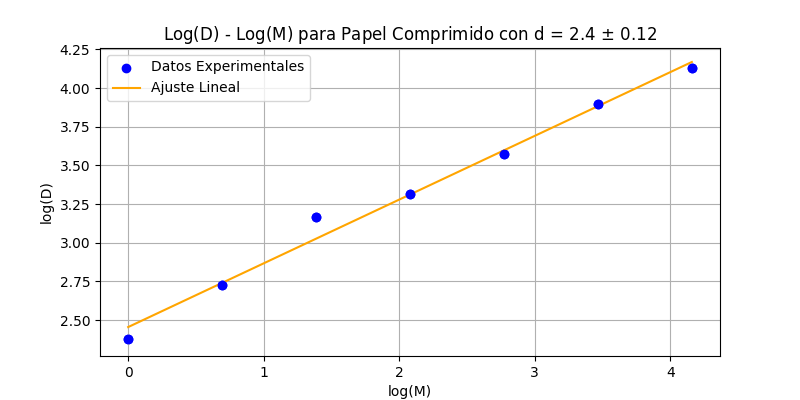
\includegraphics[width=0.4\textwidth]{Papel_comprimido_lineal.png}
    \caption{Regresión lineal para papel comprimido.}

\end{figure}

\begin{figure}[h]
    \centering
    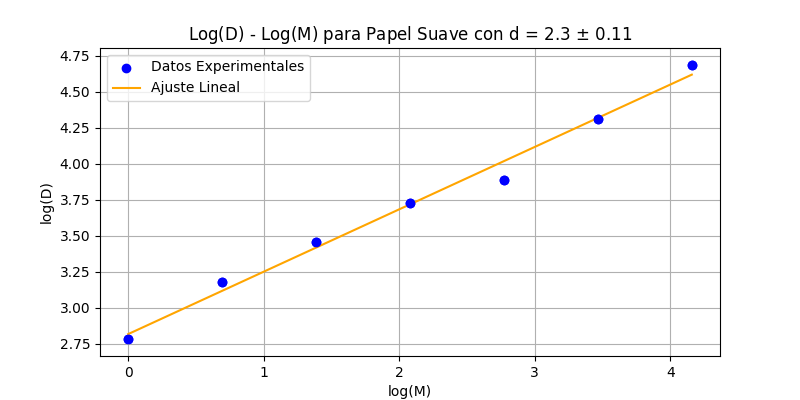
\includegraphics[width=0.4\textwidth]{Papel_suave_lineal.png}
    \caption{Regresión lineal para papel suave.}   
\end{figure}

\vspace{0.5cm}
\section{Análisis de resultados}
Además de los valores dados de dimensión fractal, se ha realizado el cálculo de residuos para cada toma
y así poder analizar la calidad del ajuste lineal realizado. Para este cálculo se ha realizado una regresión lineal 
en python con la función \texttt{scipy.stats.linregress} y a partir de esta se han obtenido los valores de 
pendiente e intercepción para cada tipo de papel y restado al valor real obtenido.

\begin{figure}[h]
    \centering
    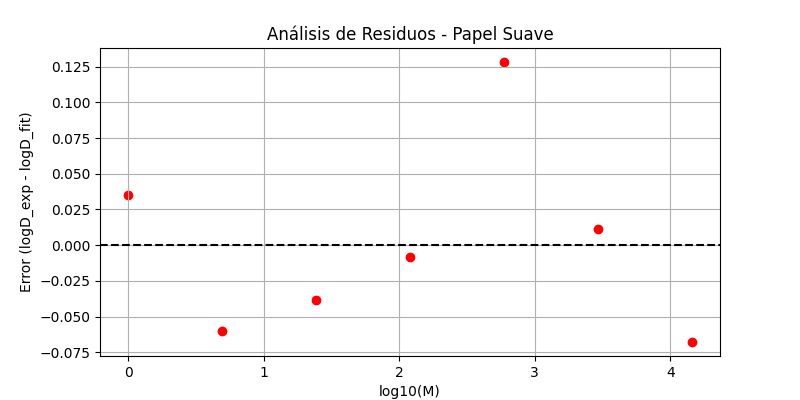
\includegraphics[width=0.4\textwidth]{Residuos_Papel_Suave.png}
    \caption{Residuos para papel suave.}
\end{figure}

\begin{figure}[h]
    \centering
    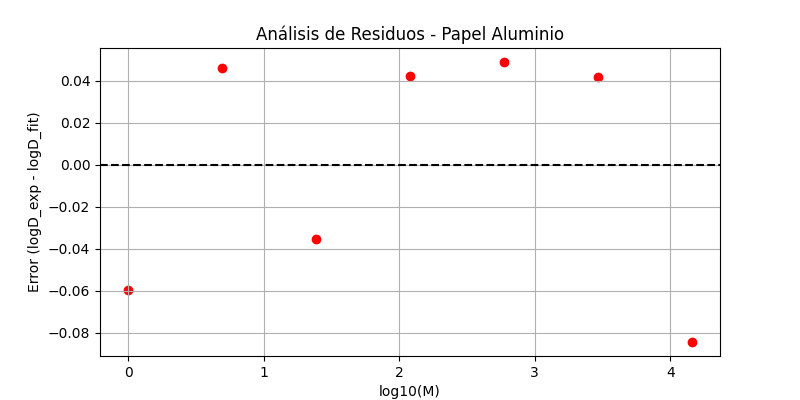
\includegraphics[width=0.4\textwidth]{Residuos_Papel_Aluminio.png}
    \caption{Residuos para papel aluminio.}
\end{figure}

\begin{figure}[h]
    \centering
    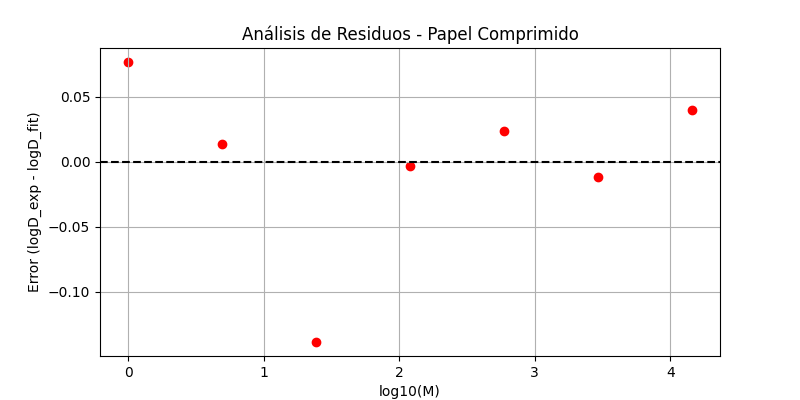
\includegraphics[width=0.4\textwidth]{Residuos_Papel_Comprimido.png}
    \caption{Residuos para papel comprimido.}
\end{figure}


\vspace{0.5cm}

Al analizar los residuos, vemos que el modelo es adecuado, si bien no representa una homostacidad perfecta ya que ciertos valores 
como el valor quinto de el papel suave tienen saltos significativos respecto a los demás.Tomando esto en cuenta, hemos comparado los resultados obtenidos con los estudios:

\vspace{0.5cm}

\cite{gomes1987fractal}, \cite{balankin2010fractal}, \cite{cambou2011three}, \cite{garcia2012bolas}.

\vspace{0.5cm}

Donde en ellos se obtiene una media de dimensión fractal de entre 2.3 a 2.5.
\vspace{0.5cm}

Vemos pues que aún a pesar de los resultados obtenidos en el cálculo de los residuos asociados a las tomas, los resultados
 experimentales son consistentes con estudios realizados previamente.

\vspace{0.5cm}

textbf{Crítica Experimental: Comparación de métodos de medida (Calibre vs. Análisis de imagen)}

Por último haremos un estudio gráfico usando el programa imageJ para medir las áreas a través de fotos y usando la relación $D_{eq} = 2\sqrt{\frac{A_{eq}}{\pi}}$ obtener los diámetros 
para el área dada por el programa. El objetivo pues de esta sección es realizar un estudio de la precisión del diámetro tomado de forma experimental.
 Para ello usaremos las siguientes fotos:

\begin{figure}[H]
    \centering
    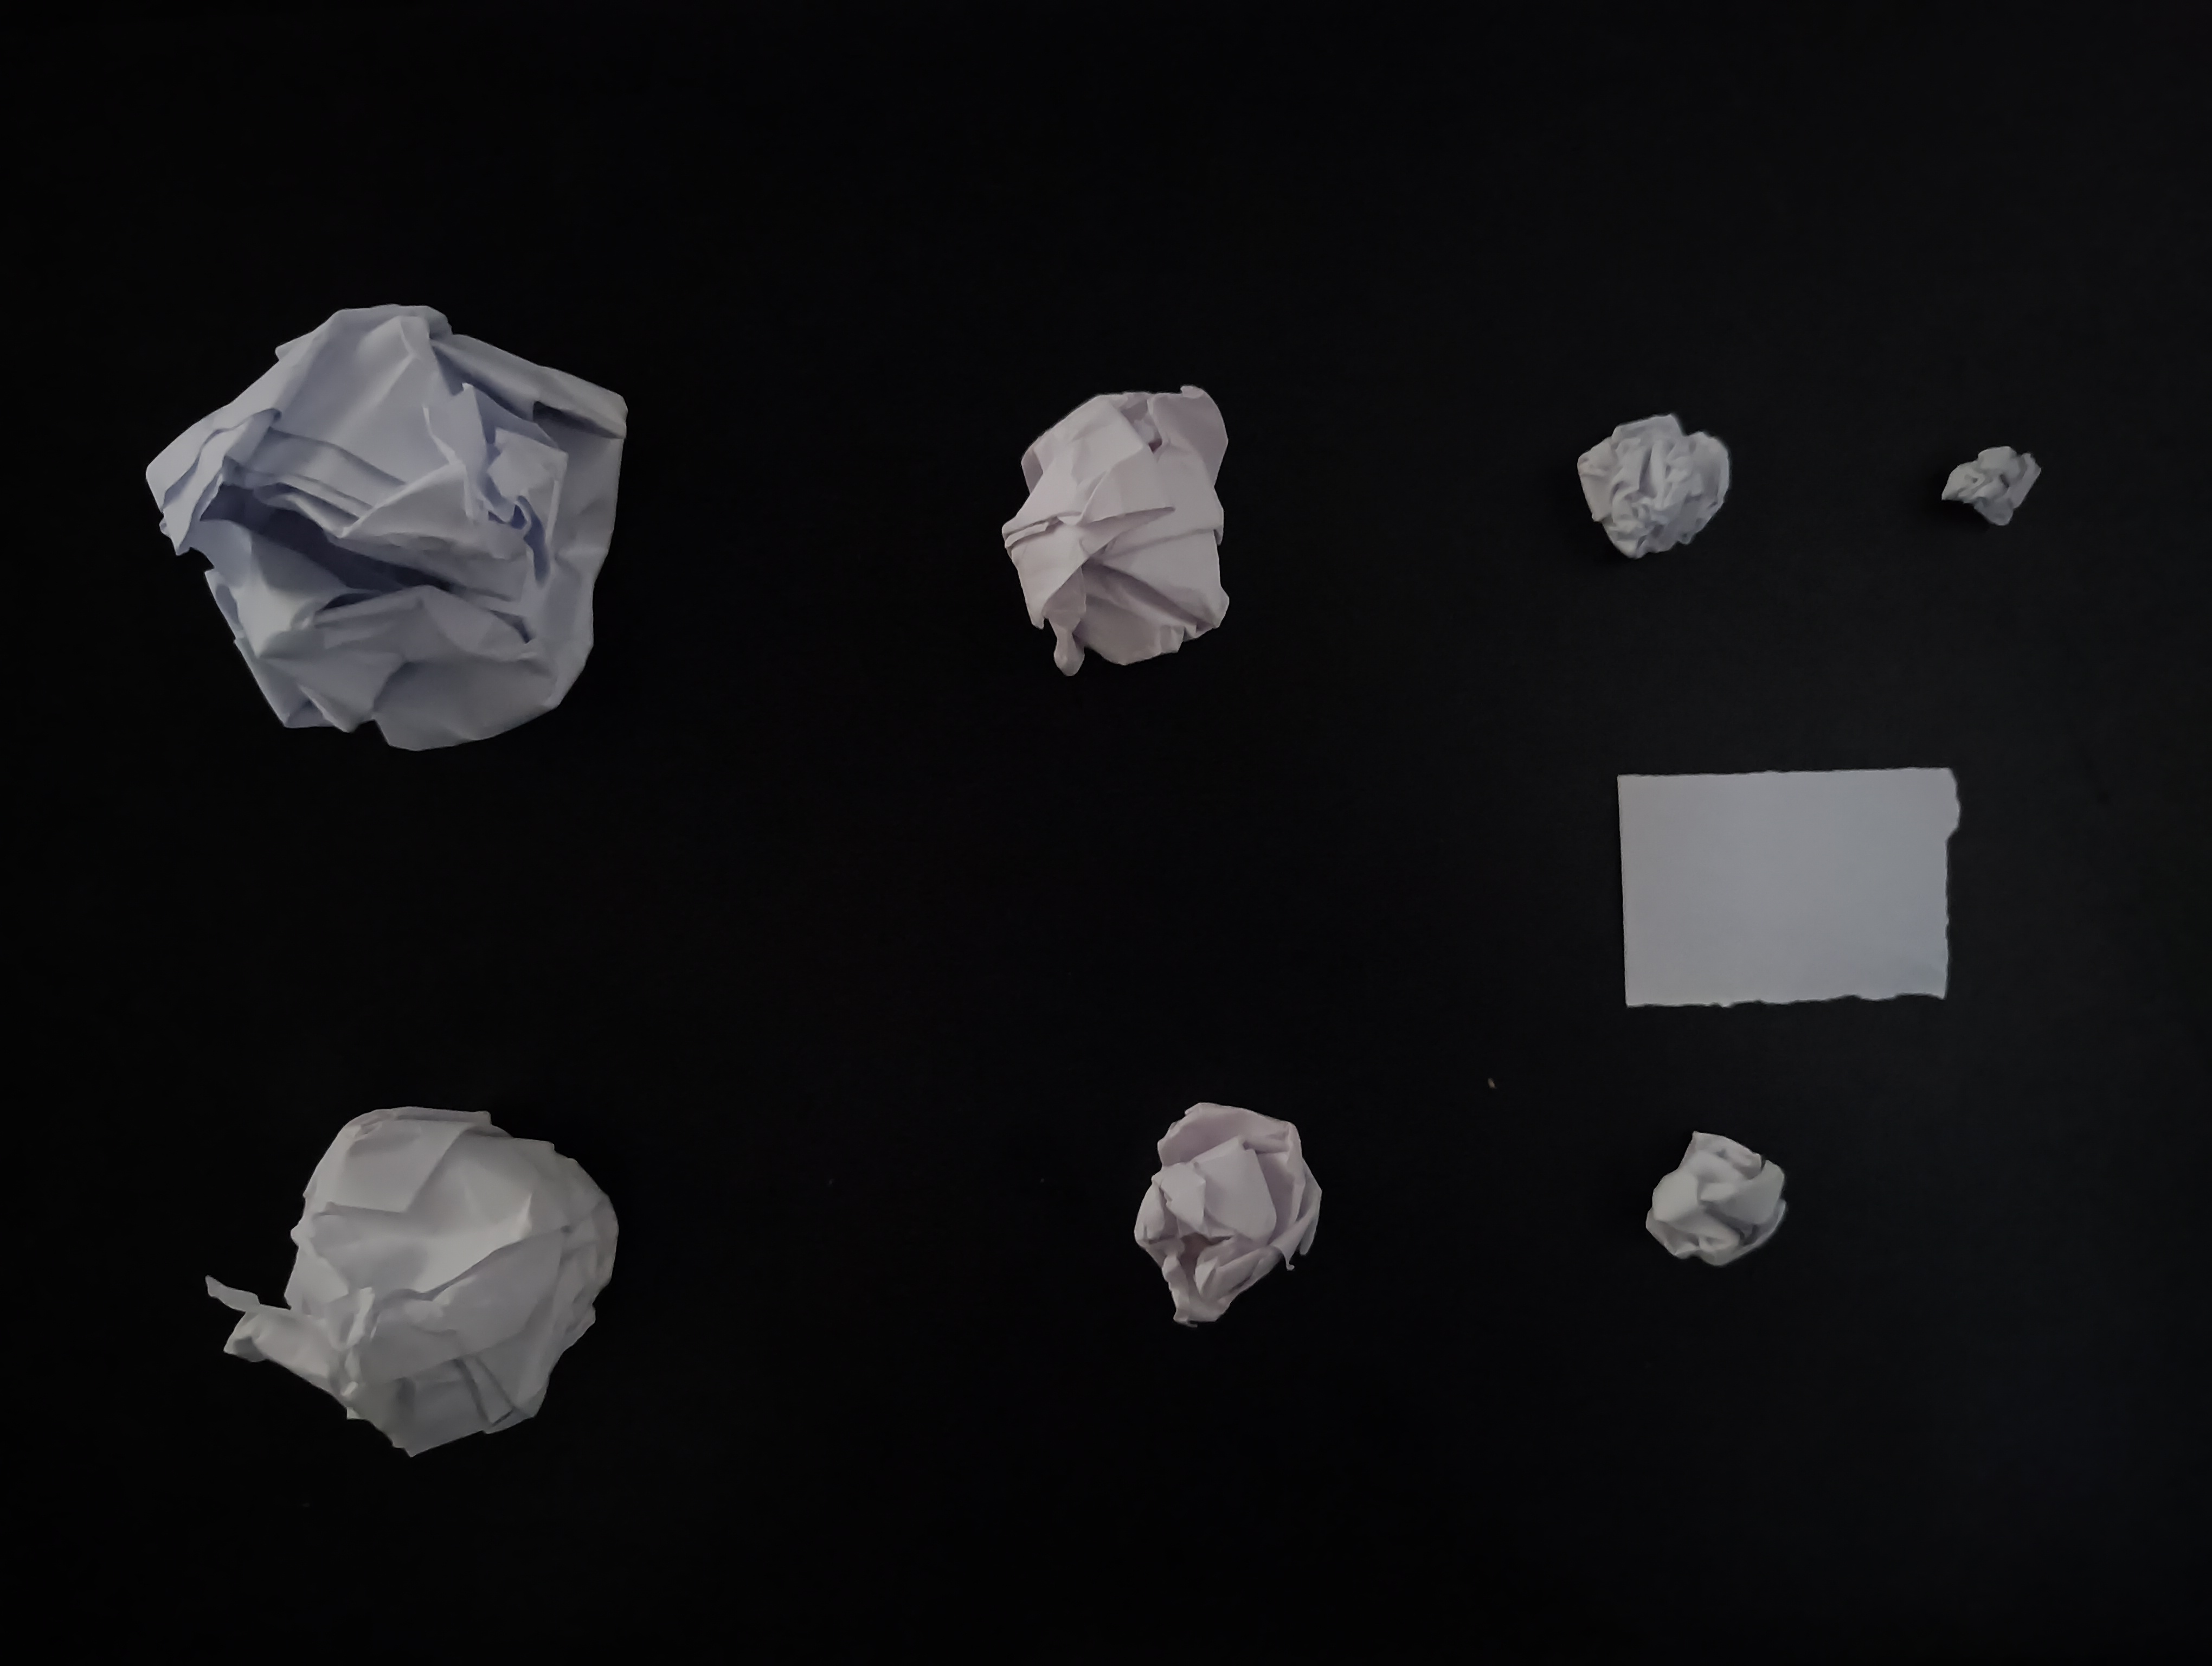
\includegraphics[width = 0.4\textwidth]{fotos_informe/papel_comprimido_real.jpg}
    \caption{Fotos del papel comprimido}
 \end{figure}
\newpage

 \begin{figure}[H]
    \centering
    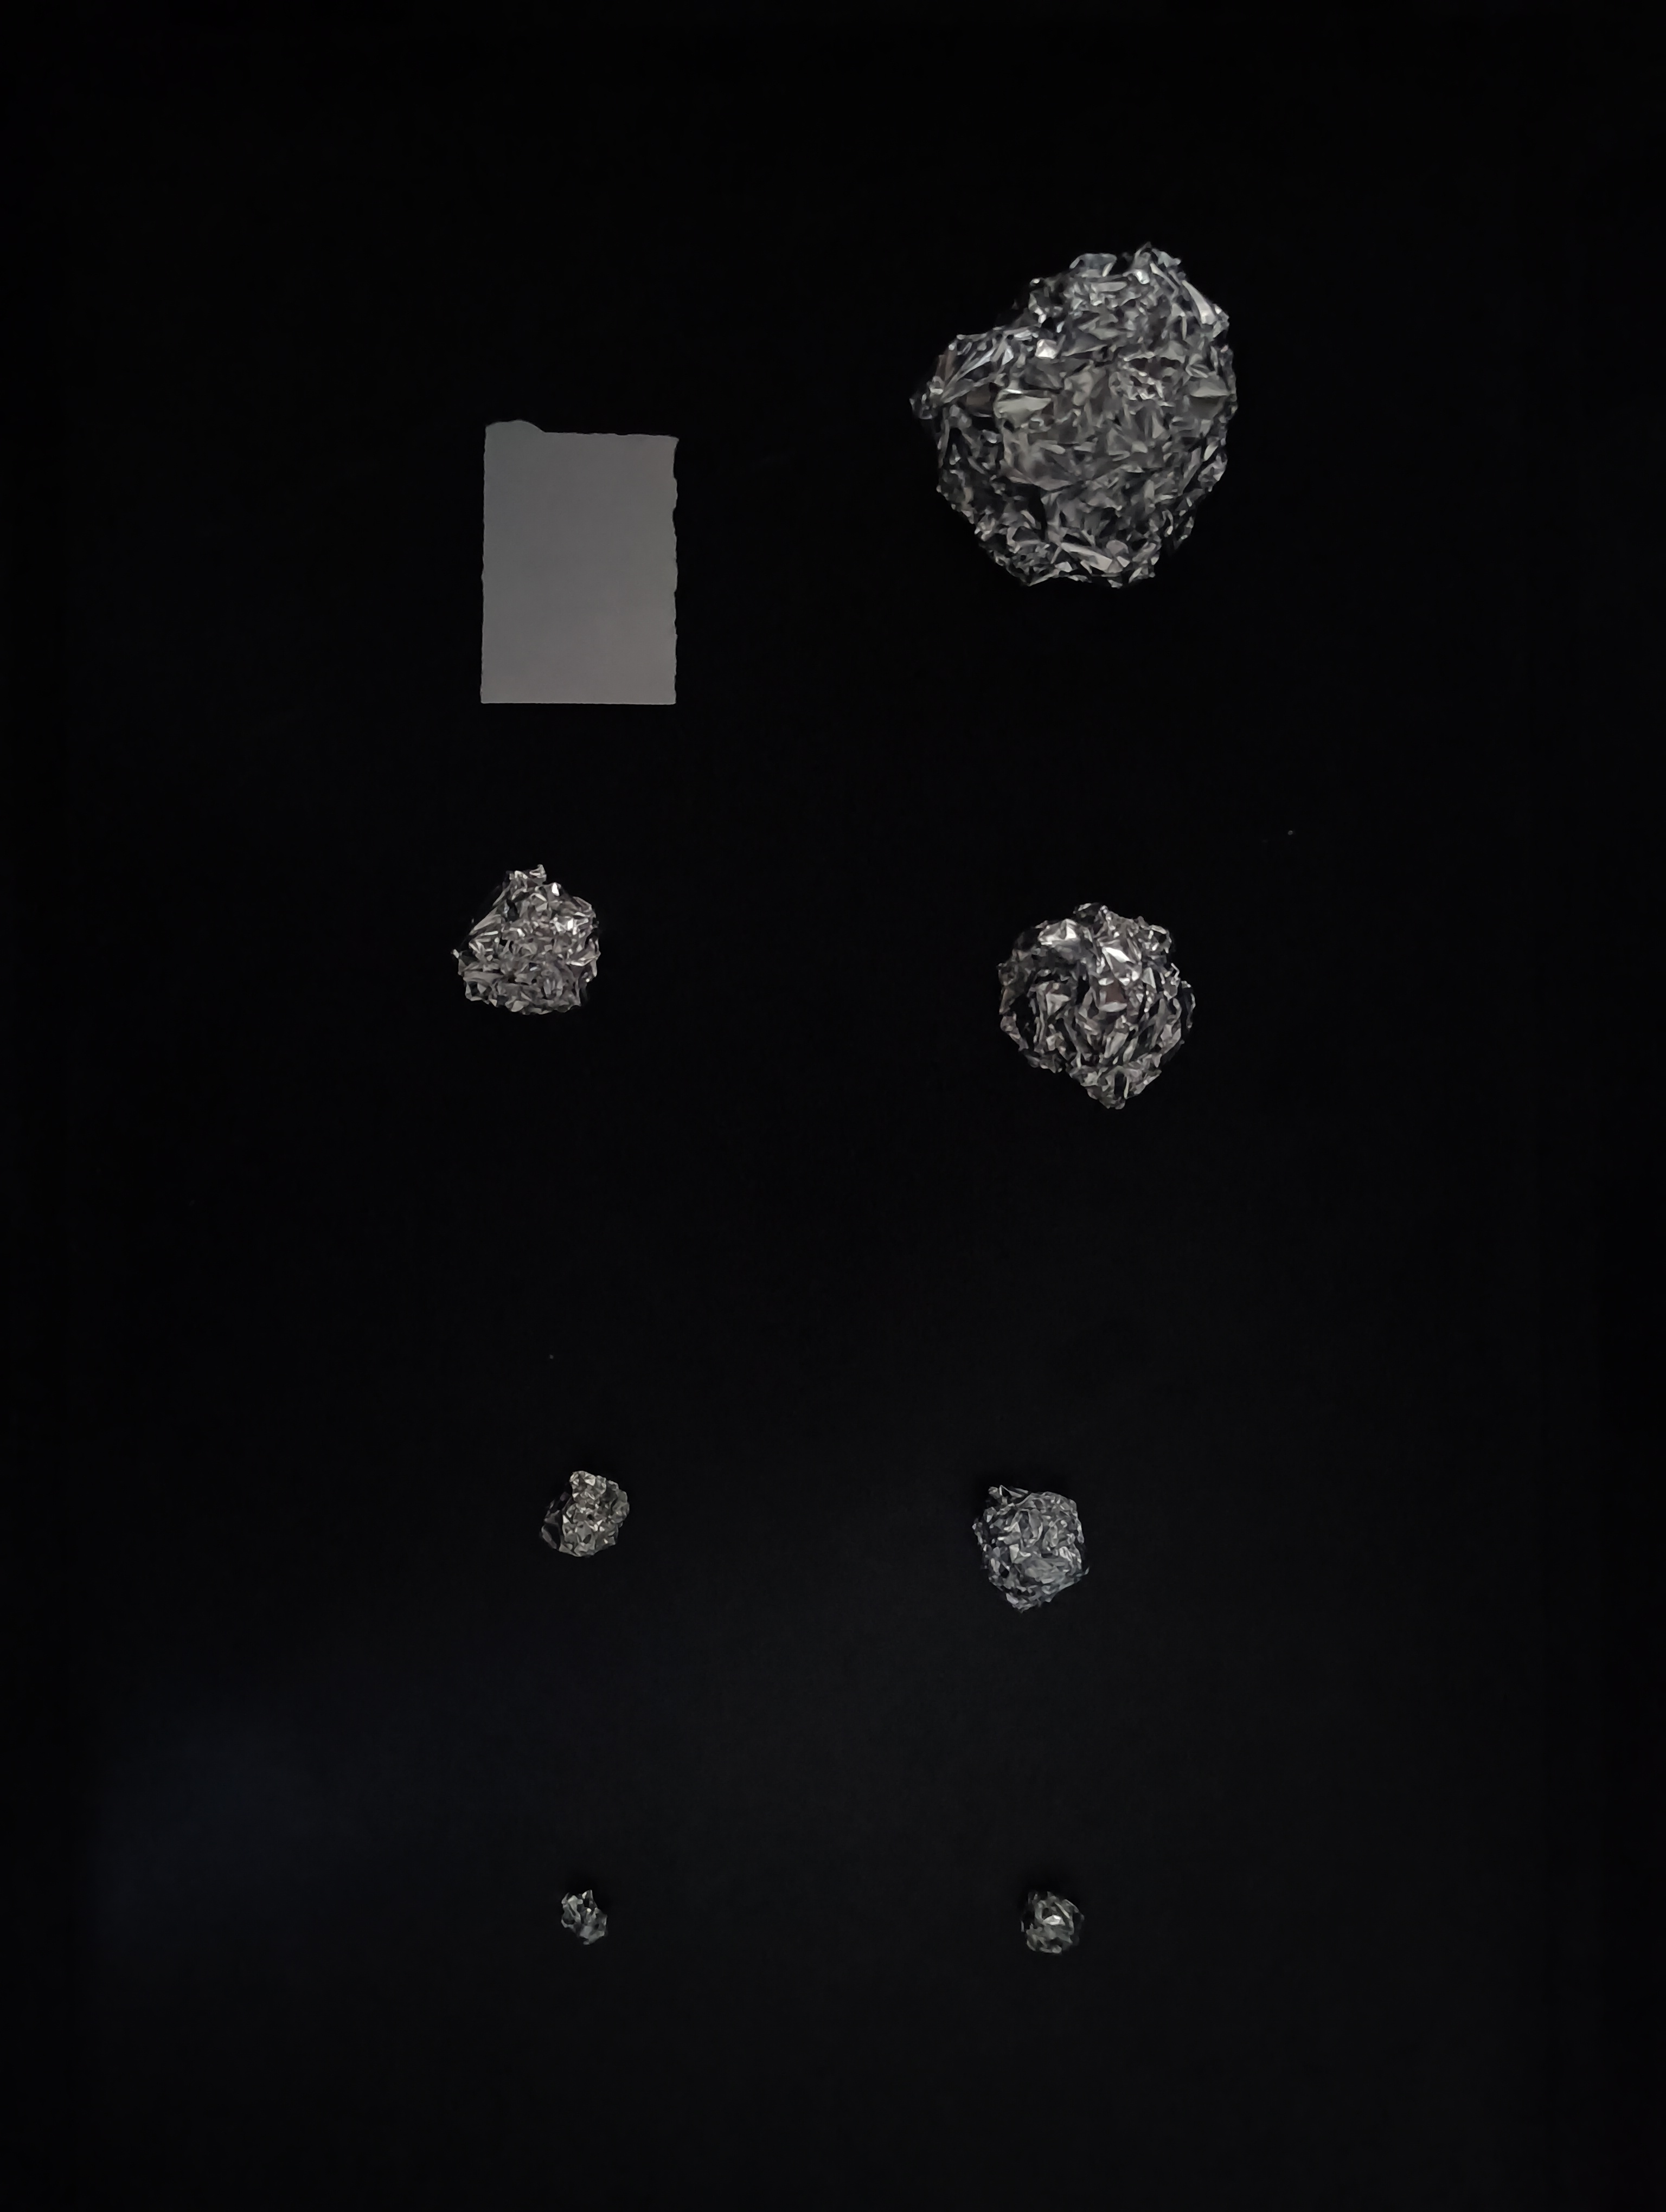
\includegraphics[width = 0.4\textwidth]{fotos_informe/papel_de_aluminio_real.jpg}
    \caption{Fotos del papel aluminio}
 \end{figure}


\begin{figure}[H]
    \centering
    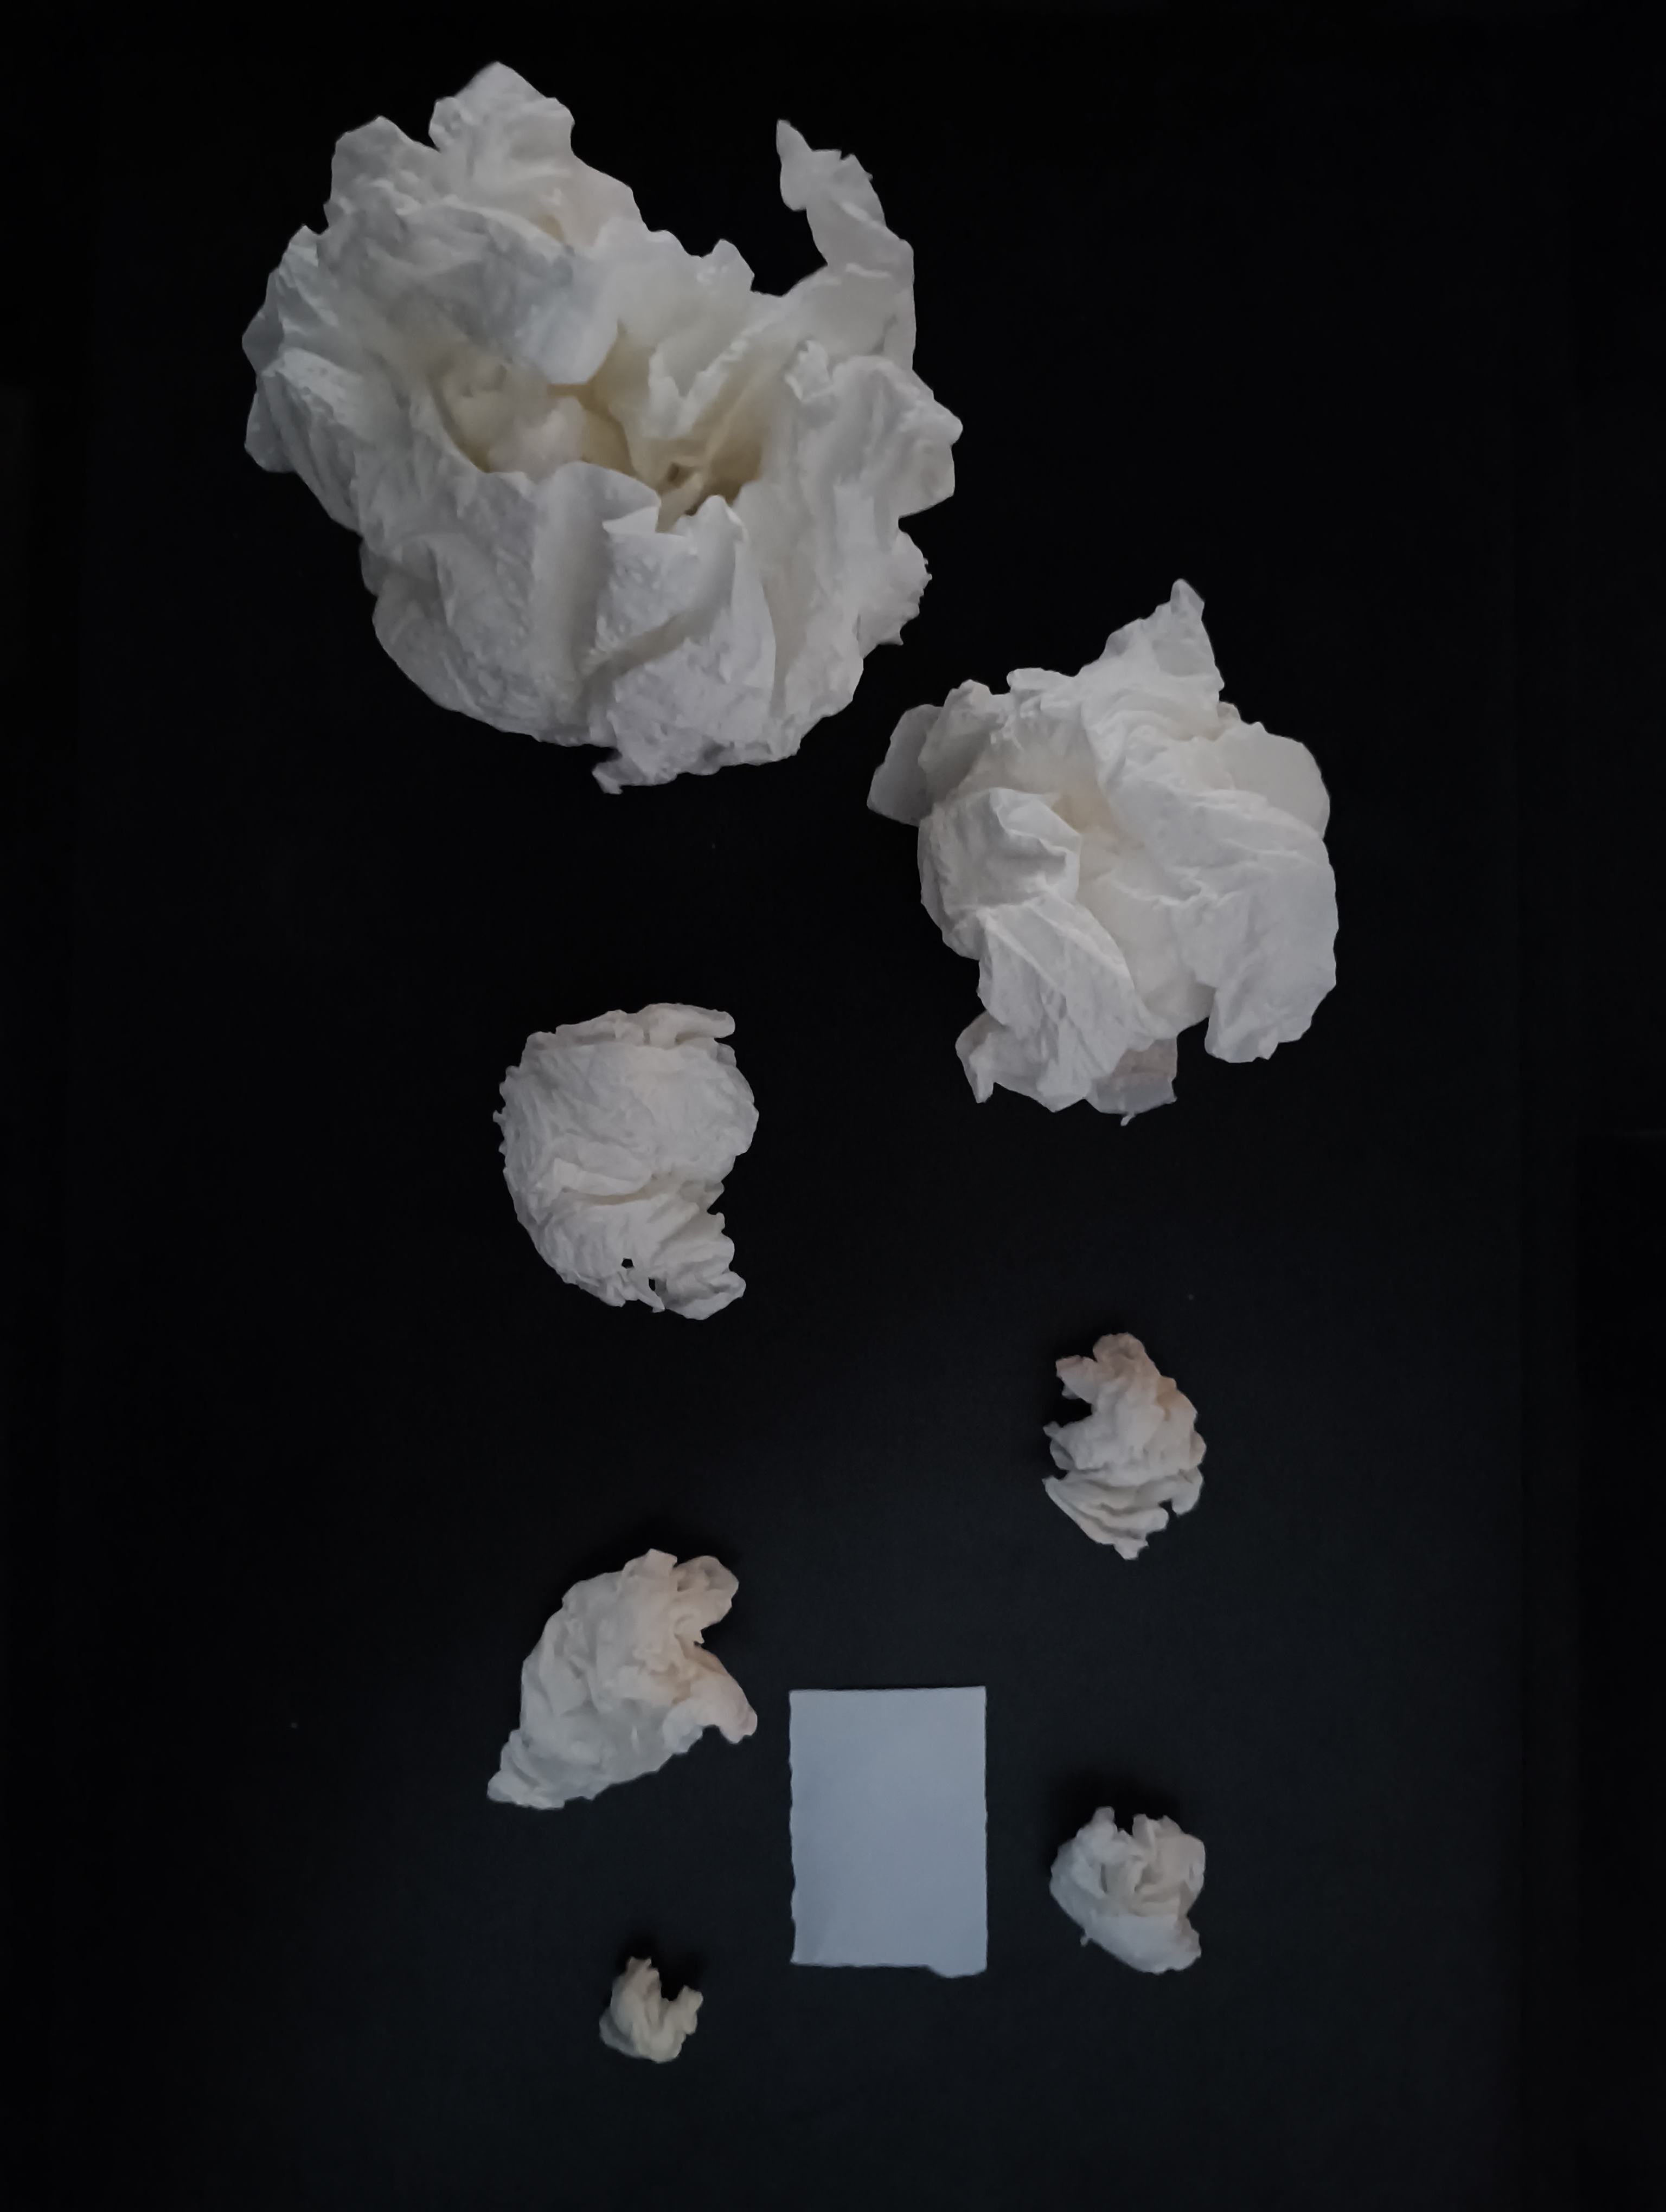
\includegraphics[width = 0.4\textwidth]{fotos_informe/papel_suave_real.jpg}
    \caption{Fotos del papel suave}
 \end{figure}

 \vspace{0.5cm}
\newpage

Estas serán procesadas en imageJ en forma de 8bit y saturando las diferentes zonas, conseguiremos una imagen que el programa puede medir en $mm^{2}$. Con ello obtenemos los siguientes
resultados: 


\begin{table}[h]
    \centering
    \small
    \begin{tabular}{ccccc}
        \toprule
        Papel   &   $m_{exp}$ &   $m_{img}$ &   $\Delta m_{exp}$ &   $\Delta m_{img}$ \\
        \midrule
        Suave      &     0.43 &     0.43 &            $\pm$ 0.02 &            $\pm$ 0.03 \\
        Aluminio   &     0.39 &     0.44 &            $\pm$ 0.01 &            $\pm$ 0.02   \\
        Comprimido &     0.41 &     0.39 &            $\pm$ 0.02 &            $\pm$ 0.02 \\
        \bottomrule
        \end{tabular}
        \caption{Comparativa de la pendiente $m$ y su error estándar $\Delta m$ obtenidos experimentalmente frente al análisis de imagen.}
        \label{tab:comparativa_errores}
\end{table}

Vemos pues que nuestros valores están considerablemente correlacionados con los obtenidos a través del análsis de imagen.
\section{Conclusiones}



Tras el estudio podemos sacar ciertas conclusiones. En primer lugar, podemos observar que la dimensión fractal siendo esta cercana a $d\approx 2.5$
se encurntra en un punto medio entre las 2D y las 3D, lo que quiere decir que no es un objeto perfectamente plano o esférico, sino que su volumen no 
ocupa todo el espacio teniendo zonas con aire lo que hace variar su volumen general. 


En el caso de que hubieramos obtenido un valor experimental de $d = 3$, eso implicaría que la bola que hemos creado sería perfectamente esférica, 
lo que implicaría que estaríamos hablando de un objeto en 3D. 

\vspace{0.5cm}
Podemos sacar otras relaciones en base a la masa y el volumen como la densidad. Como $\rho = \frac{M}{V}$ y $V \propto R^d$, 
podemos decir que $\rho \propto D^{d-3}$. Y como $d < 3$, las bolas más grandes, con mayor masa serán menos densas que las más 
pequeñas y compactas. 

\vspace{0.5cm}

Otra relación interesante es la dependendia de $d$ con el tipo de material utilizado para formar las esferas y con el método (si han sido comprimidas o no). 
En nuestro caso podemos apreciar que el pael de aluminio es el que más se acerca a tener una dimensión igual a 3, mientras que el papel no comprimido se aleja más
si bien el comprimido tiene una dimensión mayor. Es decir cuanto más maleable o más se trabaje para asimilar a una esfera, mayor será la dimensión fractal obetnida.

\vspace{1cm}
Para ver todo el análisis de datos realizado por los alumnos, se habilita este enlace al repositorio de github donde están todos los archivos de práctias: 
\cite{experimental32026}

\section{Referencias}

\nocite{gomes1987fractal}
\nocite{balankin2010fractal}
\nocite{cambou2011three}
\nocite{garcia2012bolas}

\printbibliography

\end{document}